\documentclass[fontsize=10pt]{scrartcl}

\usepackage{enumitem}
	\setenumerate{listparindent=\parindent}
\usepackage{amsmath}
\usepackage{amssymb}
\usepackage{graphicx}
\usepackage{placeins}
\usepackage{hyperref}
\usepackage{float}
\usepackage[hyphenbreaks]{breakurl}
\usepackage[margin=1.0in]{geometry}

\newcommand{\code}{\texttt}

\begin{document}

	\title{CSC 522 : Automated Learning and Data Analysis}
	\subtitle{Homework 2}
	\author{Roopak Venkatakrishnan - rvenkat7@ncsu.edu}
	\maketitle

	\section{Question 1}
	Devise a training set for use as input to the ID3 algorithm in order to produce a decision tree with a particular structure. We’re providing the required target decision tree that should be induced using your training set. In other words, instead of the usual tree induction learning problem where we’re given training data and a tree learner and we see what the program outputs, for this assignment you are given the desired output, and must design the input to produce it. To test your candidate training sets, you may use either Weka, Matlab or R.

	Construct a training set having the appropriate format for the classifier you are using, which, when used with the classifier, comes as close as you can to outputting the given decision tree. The decision tree:
\begin{verbatim}
tear-prod-rate=(normal)
| astigmatism=(yes)
| | spectacle-prescrip=(hypermetrope): none
| | spectacle-prescrip!=(hypermetrope): hard
| astigmatism!=(yes)
| | age=(presbyopic): soft
| | age!=(presbyopic): soft
tear-prod-rate!=(normal): none

\end{verbatim}

	``Outputting the tree'' means the tree structure is the same as above, with the same decision nodes in the same places, etc. Generating just any tree, no matter how accurate, is not sufficient. There must be no missing data in your training set. In other words, each example must have values for all attributes. For each example, the training set should provide values for all the following attributes, including the attributes that do not appear in the target tree. The list of attributes is given in Table 1.

	\textbf{Deliverables:} Turn in the following:
	\begin{enumerate}
	\item
	A description of how you arrived at the dataset. An answer along the lines of “I got lucky” or “this was simple trial and error” are not acceptable.

	\item
	A description of how to load the dataset in either Matlab, Weka or R, and the toolbox or package used.

	\item
	A text file with the dataset you generated.
	\end{enumerate}

	\begin{table}[H]
		\centering
	    \begin{tabular}{|c|c|}
                          \hline
	        Attributes                    & Values                            	\\ \hline \hline
	        age                           & \{young,pre-presbyopic,presbyopic\} \\ 
	        spectacle-prescrip            & \{hypermetrope,myope\}              \\ 
	        astigmatism                   & \{yes,no\}                          \\ 
	        tear-prod-rate                & \{reduced,normal\}                  \\ 
	        contact-lenses (Target Class) & \{none,soft,hard\}                  \\ 
                          \hline
                      \end{tabular}
        \caption{Table with attributes and values}
	\end{table}

	\textbf{Arriving At the dataset}

	We notice that tear-prod-rate is the root of the tree. So we try to center our values in such a way that they revolve around tear-prod-rate. The first branch says that if tear-prod-rate is reduced then the lenses required are none. We try and depict this in such a way that contact-lenses depends on nothing else but the tear-prod-rate. To achieve this we add all possible combinations of astigmatism,spectacle-prescrip and age. This way no pattern is formed here and looking at the data the ID3 algorithm is forced to say when tear-prod-rate is reduced then contact lenses is none. If we do not account for all combinations some other pattern may for unbeknown to us.

	Next we work on the other branch of the tree, where tear-prod-rate is normal. Now we see that astigmatism is the next branch. Let us consider the case where astigmatism is yes. We notice that if spectacle-prescrip=hypermetrope the contact-lense is none otherwise it is hard. So we work combinations in such way that we keep tear-prod-rate=normal, astigmatism=yes and spectacle-prescrip=hypermetrope we set cpntact-lense to none for all possible values of age. This ensures that age doesnt contribute to a pattern at this point. Next we consider tear-prod-rate=normal, astigmatism=yes and spectacle-prescrip=myope and set contact-lense=hard for all possible values of age. This makes sue that at this point the tree is split only the way we want it to be split and random patterns dont develop without our notice.

	Next we work on the branch where astigmatism is no. we consider tear-prod-rate=normal, astigmatism=no and age=presbyopic. For this we set spectacle-prescrip to all possible values and set the contact-lense=soft. This way the only pattern is that of tear-prod-rate->astigmatism->age(presbyopic). For the other two values of age (young and pre-presbyopic) we set all possible values of spectacle-prescrip for each of them. 

	We have thus constructed an ID3 algorithm in such a way that it is forced to go the way we want it to go. Because all other cases would end up with a tree of much higher length.

	The exact tree generated by my algorithm is as shown below.

\begin{verbatim}
tear-prod-rate = normal
|  astigmatism = yes
|  |  spectacle-prescrip = hypermetrope: none
|  |  spectacle-prescrip = myope: hard
|  astigmatism = no
|  |  age = pre-presbyopic: none
|  |  age = presbyopic: soft
|  |  age = young: none
tear-prod-rate = reduced: none
\end{verbatim}


	\textbf{Loading My Dataset}
	This dataset was designed to be used with Weka. The steps are as follows.
	\begin{itemize}
		\item
		Run Weka

		\item
		Click on Explorer

		\item
		Navigate to the ``Preprocess'' tab.

		\item
		Click Open-File and navigate to the file. (file-type csv)

		\item
		Go to the clasify tab, choos filter as Id3

		\item
		Make sure contact-lenses is selected in the drop down (Nom)

		\item
		leave the Test options unchanged. and click start

		\item
		Result is produced on the classifier output box in the same tab.
	\end{itemize}
	\section{Question 2}

		\begin{sloppypar}
		For this exercise, we will use the Balloons dataset (\url{http://archive.ics.uci.edu/ml/datasets/Balloons}). Specifically, we will use the yellow-small+adult-stretch data. (\burl{http://archive.ics.uci.edu/ml/machine-learning-databases/balloons/yellow-small+adult-stretch.data}).
		\end{sloppypar}
		The data has 16 entries each four attributes, all of which are nominal. Each entry belongs to one of the two classes {T, F}. Complete the following tasks.

		\begin{enumerate}
			\item
			Compute the tree using Gini index. Show all necessary calculations.

\begin{verbatim}
> vals<-read.csv(file.choose())
> names(vals)<- c("color","size","act","age","inflated")
> findgini <- function (vals, inflated) {
+   
+   
+     unq <- unique(vals)
+     gini <- c()
+     df <- data.frame(v=vals,inf=inflated)
+     gini_final<-0
+     for(i in 1:length(unq))
+     {
+       no_type_i <- length(vals[which(vals==unq[i])])
+       no_true <- length(which(inflated[which(vals==unq[i])]))
+       no_false <- no_type_i - no_true
+       tmp = 1 -(no_true/no_type_i)^2 -(no_false/no_type_i)^2
+       tlength <-length(vals)
+       gini_final<-gini_final + ((no_type_i/tlength)*tmp)
+     }
+     print(paste("The Gini is ",gini_final))
+   
+ 
+ }
> findgini(vals$color,vals$inflated)
[1] "The Gini is  0.421875"
> findgini(vals$size,vals$inflated)
[1] "The Gini is  0.421875"
> findgini(vals$act,vals$inflated)
[1] "The Gini is  0.421875"
> findgini(vals$age,vals$inflated)
[1] "The Gini is  0.421875"
> findgini(vals$size[which(vals$color=="YELLOW")],
+ vals$inflated[which(vals$color=="YELLOW")])
[1] "The Gini is  0.1875"
> findgini(vals$act[which(vals$color=="YELLOW")],
+ vals$inflated[which(vals$color=="YELLOW")])
[1] "The Gini is  0.4375"
> findgini(vals$age[which(vals$color=="YELLOW")],
+ vals$inflated[which(vals$color=="YELLOW")])
[1] "The Gini is  0.4375"
> findgini(vals$size[which(vals$color=="PURPLE")],
+ vals$inflated[which(vals$color=="PURPLE")])
[1] "The Gini is  0.375"
> findgini(vals$act[which(vals$color=="PURPLE")],
+ vals$inflated[which(vals$color=="PURPLE")])
[1] "The Gini is  0.25"
> findgini(vals$age[which(vals$color=="PURPLE")],
+ vals$inflated[which(vals$color=="PURPLE")])
[1] "The Gini is  0.25"
> findgini(vals$act[intersect(which(vals$color=="YELLOW"),
+ which(vals$size=="SMALL"))],
+ vals$inflated[intersect(which(vals$color=="YELLOW"),
+ which(vals$size=="SMALL"))])
[1] "The Gini is  0"
> findgini(vals$act[intersect(which(vals$color=="YELLOW"),
+ which(vals$size=="LARGE"))],
+ vals$inflated[intersect(which(vals$color=="YELLOW"),
+ which(vals$size=="LARGE"))])
[1] "The Gini is  0.25"
> findgini(vals$age[intersect(which(vals$color=="YELLOW"),
+ which(vals$size=="LARGE"))],
+ vals$inflated[intersect(which(vals$color=="YELLOW"),
+ which(vals$size=="LARGE"))])
[1] "The Gini is  0.25"
> findgini(vals$age[intersect(which(vals$color=="YELLOW"),
+ which(vals$size=="SMALL"))],
+ vals$inflated[intersect(which(vals$color=="YELLOW"),
+ which(vals$size=="SMALL"))])
[1] "The Gini is  0"
> findgini(vals$age[intersect(which(vals$color=="YELLOW"),
+ which(vals$size=="LARGE"))],
+ vals$inflated[intersect(which(vals$color=="YELLOW"),
+ which(vals$size=="LARGE"))])
[1] "The Gini is  0.25"
> findgini(vals$size[intersect(which(vals$color=="PURPLE"),
+ which(vals$act=="STRETCH"))],
+ vals$inflated[intersect(which(vals$color=="PURPLE"),
+ which(vals$act=="STRETCH"))])
[1] "The Gini is  0.5"
> findgini(vals$age[intersect(which(vals$color=="PURPLE"),
+ which(vals$act=="STRETCH"))],
+ vals$inflated[intersect(which(vals$color=="PURPLE"),
+ which(vals$act=="STRETCH"))])
[1] "The Gini is  0"
> findgini(vals$age[intersect(which(vals$color=="PURPLE"),
+ which(vals$act=="DIP"))],
+ vals$inflated[intersect(which(vals$color=="PURPLE"),
+ which(vals$act=="DIP"))])
[1] "The Gini is  0"
> findgini(vals$act[intersect(which(vals$color=="PURPLE"),
+ which(vals$act=="DIP"))],
+ vals$inflated[intersect(which(vals$color=="PURPLE"),
+ which(vals$act=="DIP"))])
[1] "The Gini is  0"
\end{verbatim}
			Let us use the above function and the data to construct a decision tree. This function computes the Gini value given the corresponding values and the respective output expected.

			First we see wehere we get the lowest $GINI_{split}$ trying all columns. In this case we notice that all the columns give us a value of $GINI_{split} = 0.421875$. This value is calculated by the above written fucntion.\\
			Let us run through how the function calculates the $GINI_{split}$. First it finds GINI for each of the different values of the column passed. Let us consider as an exmaple. It has two different values, YELLOW and PURPLE. Let us now calulate GINI(color=YELLOW).

			This can be found as 
			\begin{equation*}
				1 - (\frac{5}{8})^{2} - (\frac{3}{8})^{2}
			\end{equation*}

			Similarly  we find the GINI value for PURPLE

			Combining both the values given we find the value for $GINI_{split} (Color)$

			Since our function does the abve steps we can use the value it gives us and move forward quicker.

			Since all seem to have the same level of impurity in the firts level, let us just pick color move on.\\
			Now we try and see what happens for color = YELLOW and size,act,age. We see the following.\\


			Given COLOR=YELLOW, $GINI_{split}$ is given to be
			\[   \left\{
                  \begin{array}{ll}
                        0.1875 & size \\
                        0.4375 & act \\
                        0.4375 & age \\
                  \end{array} 
                  \right. \]
			
			Given COLOR =PURPLE, $GINI_{split}$ is given to be
			\[   \left\{
                  \begin{array}{ll}
                        0.375 & size \\
                        0.25 & act \\
                        0.25 & age \\
                  \end{array} 
                  \right. \]
            Given the above we can see the best partition would be along size for COLOR=YELLOW and either of act/age for COLOR=PURPLE. Let us choose to proceed with act for PURPLE

            Given COLOR=YELLOW, SIZE=LARGE, $GINI_{split}$ is found to be
            \[   \left\{
                  \begin{array}{ll}
                        0.25 & act \\
                        0.25 & age \\
                  \end{array} 
                  \right. \]
            Thus since both are identical we can choose either and proceed. From this point onward we find the GINI values to be 0. So we proceed to draw the tree.

            Given COLOR=PURPLE,act=STRETCH, $GINI_{split}$ is found to be
             \[   \left\{
                  \begin{array}{ll}
                        0.5 & size \\
                        0.0 & age \\
                  \end{array} 
                  \right. \]
            Here we choose age and finalize the tree. 

            The final tree we construct looks as follows. \\
            \begin{figure}[H]
				\begin{center}
					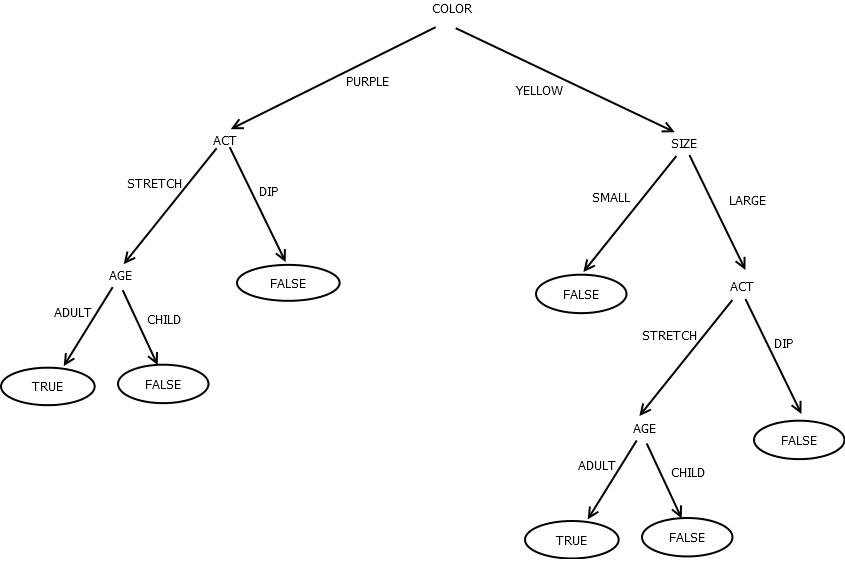
\includegraphics[width=\textwidth]{resources/q2_img1.png}
					\caption{Decision Tree - GINI index}
				\end{center}
			\end{figure}
		\end{enumerate}
\end{document}